\documentclass[a4paper, 12pt]{report}

\title{Éditeur web}
\author{Pierre Burc, Olivier Duplouy, Hamza Erraji, Issame Amal, Mickaël Berger, Joachim Divet, Zaydane Sadiki & Abdelhamid Belarbi}

%% Pour des marges plus équitables.
\usepackage[margin=1.5cm]{geometry}
%% Pour la langue des titres et sous-titres.
\usepackage[francais]{babel}
%% Pour de belles images.
\usepackage{graphicx}
%% Pour la police de caractères.
\usepackage{fontspec}
\setmainfont{Delicious-Roman}
%% Pour faire le glossaire.
\usepackage[xindy]{glossaries}
\makeglossaries
%% Pour les notes de bas de page.
\usepackage{fmtcount}
\begin{document}
	%% Glossaire
	\newglossaryentry{UML}
	{
		name={UML},
		description={Unified Modeling Language, langage de modélisation graphique à base de pictogrammes}
	}

	\newglossaryentry{diagramme de Gantt}
	{
		name={diagramme de Gantt},
		description={Le diagramme de Gantt est un outil utilisé en ordonnancement et gestion de projet et permettant de visualiser dans le temps
		les diverses tâches liées composant un projet. Il permet de représenter graphiquement l'avancement du projet}
	}
	
	\newglossaryentry{bogue}
	{
		name={bogue},
		description={En informatique, un bug (de l’anglais bug, « insecte ») ou bogue est un défaut de conception d'un programme
		informatique à l'origine d'un dysfonctionnement},
		plural={bogues}
	}
		
	\newglossaryentry{Qt}
	{
		name={Qt},
		description={Qt est un framework orienté objet et développé en C++. Il offre des composants d'interface graphique (widgets),
		d'accès aux données, de connexions réseaux, de gestion des fils d'exécution, d'analyse XML, etc}
	}

	\newglossaryentry{gestionnaire de version}
	{
		name={gestionnaire de version},
		description={La gestion de versions consiste à maintenir l'ensemble des versions d'un ou plusieurs fichiers (généralement en texte).
		Essentiellement utilisée dans le domaine de la création de logiciels, elle concerne surtout la gestion des codes source}
	}

	\newglossaryentry{Git}
	{
		name={Git},
		description={Git est un logiciel de gestion de versions décentralisé. 
		C'est un logiciel libre créé par Linus Torvalds, le créateur du noyau Linux, et distribué selon les termes de la licence 
		publique générale GNU version 2}
	}

	\newglossaryentry{WYSIWYG}
	{
		name={WYSIWYG},
		description={Un WYSIWYG est une interface utilisateur qui permet de composer visuellement le résultat voulu, typiquement 
		pour un logiciel de mise en page, un traitement de texte ou d’image. 
		C'est une interface « intuitive » : l’utilisateur voit directement à l’écran à quoi ressemblera le résultat final}
	}
	
	\newglossaryentry{autocomplétion}
	{
		name={autocomplétion},
		description={l'autocomplétion, est une fonctionnalité informatique permettant à l'utilisateur de limiter la quantité d'informations 
		qu'il saisit avec son clavier, en se voyant proposer un complément qui pourrait convenir à la chaîne de caractères qu'il a commencé à taper}
	}

	\newglossaryentry{expression régulière}
	{
		name={expression régulière},
		description={Une expression rationnelle ou expression régulière est en informatique une chaîne de caractères que l’on appelle parfois un motif
		et qui décrit un ensemble de chaînes de caractères possibles selon une syntaxe précise.
		Les expressions rationnelles sont issues des théories mathématiques des langages formels},
		plural={expressions régulières}
	}

	\begin{titlepage}
		\center{
\includegraphics[width=5cm]{images/logoUM2.png}}\\ 
		~\\
		~\\
		~\\
		~\\
		~\\		
		\begin{center}
			{\large Rapport de projet} \\
			{\large Licence 3}\\
			\vspace{1,5cm}
			{\Huge Editeur de sites web}\\
			~\\
			~\\
			~\\
			
\includegraphics[width=12.5cm]{images/logoTest1.png}
			~\\
			~\\
			{\large Réalisé par :} \\
			~\\
			{\LARGE Pierre Burc, Olivier Duplouy, \\
				      Hamza Erraji, Issame Amal,\\
				      Mickaël Berger, Joachim Divet,\\
				      Zaydane Sadiki et Abdelhamid Belarbi}\\
			\vspace{1,5cm}
			{\large Sous la direction de:} \\
			~\\
			{\LARGE Michel Meynard} \\
			\vspace{2.5cm}
			{\large Année universitaire 2011-2012 }			
		\end{center}
	\end{titlepage}
%%%%%%%%%%%%%%%%%%%%%%%%%%%%%%%%%%%%%%%%
%%%%%%%%%%%%%%%%%%%%%%%%%%%%%%%%%%%%%%%%
	\begin{chapter}*{Remerciements}
	Nous tenons à remercier tout particulièrement M. Michel Meynard, notre tuteur de projet qui nous a guidés et épaulés tout au long de
	ces quelques mois de travail, égrénant ça et là différents conseils utiles à souhait. \\

	Bien entendu nous n'oublions pas de remercier chaleureusement toute l'équipe pédagogique de l'UM2 qui nous a apporté son soutien.\\

	Et il va sans dire que tous les membres du groupe se remercient les uns les autres.
	\end{chapter} 
%%%%%%%%%%%%%%%%%%%%%%%%%%%%%%%%%%%%%%%%
%%%%%%%%%%%%%%%%%%%%%%%%%%%%%%%%%%%%%%%%
	%% Table des matières.
	\tableofcontents
	%% Table des figures
	\listoffigures
%%%%%%%%%%%%%%%%%%%%%%%%%%%%%%%%%%%%%%%%
%%%%%%%%%%%%%%%%%%%%%%%%%%%%%%%%%%%%%%%%
	\begin{chapter}*{Introduction}
	\addcontentsline{toc}{chapter}{Introduction}

	% 	Au début du mois de Février, il nous a été demandé de réaliser un projet ayant pour but de mettre en place une application permettant
	% d'utiliser un éditeur multi-fichiers effectuant différentes actions sur des fichiers relatif à un site web.\\
	% Ce dernier consiste à créer, modifier, sauvergarder... des fichiers contenant les langages JavaScript, HTML, CSS, PHP via une interface se
	% rapprochant des IDEs présents sur le marché. Celle-ci aura un rôle primordial, car elle devra apporter à l'utilisateur une aide précieuse grâce
	% à des fonctionnalités intuitives, comme par exemple l'autocomplétion.\\
	% A l'occasion de ce projet, un groupe de huit personnes a été formé pour répondre à la capacité de travail demandée. Nous devions donc nous 
	% répartir les tâches entre chaque membre voir créer des sous-groupes permettant de cloisonner chaque brique essentielle de l'application 
	% (interface,système,coloration/complétion). De plus, une période de trois mois nous a été accordée pour réaliser cet IDE.\\
	% Afin de ne pas gaspiller du temps à déterminer par où commencer et de quelle façon aborder le sujet, nous avions des réunions régulières avec 
	% notre tuteur M.Meynard, pour nous guider dans notre réflexion.\\
	% A travers ce compte-rendu nous essaierons de rendre compte des étapes qui nous ont conduits à élaborer cette application en essayant de répondre 
	% le plus fidèlement possible au problème posé.\\ 

	C'est par une froide journée d'hiver que nous nous réunîmes pour la première fois à l'université de Montpellier. 
	Huit, tous étudiants préposés au projet numéro vingt-trois nous attendons à notre table l'arrivée de notre tuteur M. Meynard. 
	Ce dernier se présente, nous salue et prononce ce discours mémorable qui restera gravé dans nos mémoires.\\
	\begin{quotation}
		``Dans le cadre de développement de sites Web, on souhaiterait utiliser un éditeur multi-fichiers permettant de réaliser différentes actions sur
		des fichiers relatifs à un site: édition de fichiers Html, Php, JavaScript et Css.

		Il serait également appréciable que cet éditeur proposât un mode de visualisation du site dans un navigateur et un mode arborescence.

		On pourrait aussi avoir de l'\gls{autocomplétion}, de la coloration syntaxique, un accès aux manuels des langages cités précédemment et pourquoi
		pas une validation Html.\,''
	\end{quotation}

	Après ce laïus prononcé d'une traite M. Meynard disparut soudain, nous laissant là, le regard vide.\\


	Néanmoins, nous nous remîmes assez vite de notre ahurissement et un sage parmi nous s'écria soudain:
	\begin{quotation}
		``Nous commencerons par étudier quelques éditeurs existants sur le marché pour nous faire une idée. Ensuite nous concevrons
		le programme avec le langage UML en nous organisant pour la réalisation.
		Enfin, nous implémenterons l'application insolents et sûrs de nous.	Qu'en dites-vous ?''
	\end{quotation}

	Nous n'en dîmes que du bien. En effet, l'idée loin d'être incroyablement novatrice avait l'avantage d'être logique et cohérente.\\


	C'est ainsi que démarra le projet \emph{Éditeur web} décrit dans ce document, entrons donc sans plus attendre dans le vif du sujet.
	
	\end{chapter}
%%%%%%%%%%%%%%%%%%%%%%%%%%%%%%%%%%%%%%%%
%%%%%%%%%%%%%%%%%%%%%%%%%%%%%%%%%%%%%%%%
	\begin{part}{Analyse}
		\begin{chapter}{Cahier des charges}
			Voici une liste exhaustive des fonctionnalités prescrites par M. Meynard:
			\begin{itemize}
				\item Édition des fichiers JavaScript, Php, Css et Html;
				\item Un système multi-onglets permettant de naviguer rapidement entre plusieurs fichiers d'un même projet;
				\item Possibilité de visualiser le site sous forme d'arborescence;
				\item Mode \gls{autocomplétion} et coloration syntaxique;
				\item Mode auto-indentation;
				\item Accès en un clic au manuel Php/Html/Css/JavaScript;
				\item Validation Html;
				\item Visualisation du site dans un navigateur;
				\item Squelette de site préexistant.
			\end{itemize}~\\

			La liste d'exigences ci dessus se résume en une besoins graphiques, il nous fallait donc ``deviner'' ce qui se déroule en interne 
			dans le programme. Malgré les différents avis données par M. Meynard, il était difficile pour la majorité des membres de
			comprendre comment fonctionnait un tel programme.\\

			Après plusieurs colloques, discussions, palabres et réunions, il fut décidé que le meilleur moyen de se rendre compte de ce que
			représentait un tel cahier des charges en terme de produit fini était d'étudier les différents éditeurs existants offrants ce 
			genre de fonctionnalités.
		\end{chapter}

		\begin{chapter}{Étude de projets existants}
		\begin{section}{Espresso}
				\begin{figure}[h]
					\begin{center}
						
\includegraphics[width=3cm]{images/logoEspresso.png}
						\caption{Espresso}
					\end{center}
				\end{figure}~\\
				Le premier programme d'édition de site web que nous avons étudié propose les mêmes fonctionnalités que le
				logiciel que nous nous proposons de développer, à savoir coloration syntaxique, indentation automatique, arborescence des codes, etc.
				Il sera à priori une bonne source d'inspiration pour nous d'autant plus que l'interface est très soignée et agréable d'utilisation.
			\end{section}
			~\\
			\begin{section}{Aptana}
				\begin{figure}[h]
					\begin{center}
						
\includegraphics[width=4cm]{images/logoAptana.png}
						\caption{Aptana}
					\end{center}
				\end{figure}~\\
				Cet éditeur propose un ensemble de fonctionnalités nombreuses et variées. 
				Beaucoup plus fourni que Espresso, il propose des fonctionnalités complexes dans divers langages : 
				déboguage, déploiement automatique, gestionnaire de version inclus, terminal intégré et moult autres outils.
				Pour nous c'est un bon modèle à suivre en évitant tout de même de tomber dans le piège du sur-nombre d'options 
				qui importuneraient l'utilisateur. 
			\end{section}
			~\\
			\begin{section}{Dreamweaver}
				\begin{figure}[h]
					\begin{center}
						
\includegraphics[width=3cm]{images/logoDreamweaver.png}
						\caption{Dreamweaver}
					\end{center}
				\end{figure}~\\
				Dreamweaver est une référence en la matière. Il réunit les atouts des deux éditeurs sus-cités en joignant l'utile à l'agréable.
				Il possède en outre un mode dit \gls{WYSIWYG} permettant de dessiner l'interface d'un site web.
			\end{section}
			~\\


			\begin{section}{Bilan comparatif}
				Le tableau \ref{comparatif}, donne la distributions de quelques fonctionnalités parmi les logiciels cités précédemment. Il est
				inutile de mettre dans ce tableau des fonctionnalités telles que la coloration ou l'édition de fichier, car il est évident que des
				lesdits logiciels possèdent ce genre de spécificités.\\

				%% Ajout d'une petite note de bas de page.
				\addtocounter{footnote}{1}
				\footnotetext[\value{footnote}]{À noter que l'auto-indentation dans le tableau \ref{comparatif} concerne la capacité de 
				formater tout un fichier et non pas d'ajouter une tabulation après saut de ligne.}
				\begin{table}[h]
				\caption{\label{comparatif} Fonctionnalités spéciales dans les éditeurs étudiés}
					\begin{tabular}{|c||c|c|c|c|c|} % c signifie center, le texte de chaque colonne sera donc centré.
					  \hline
					  Éditeur & onglets & autocomplétion & auto-indentation$^{\decimal{footnote}}$ & validation Html & documentations \\
					  \hline

					  Espresso & oui & oui & non & non & non \\
					  Aptana & oui & oui & non & oui & oui \\
					  Dreamweaver & oui & oui & oui & oui & non \\
					  \hline
					\end{tabular}
				\end{table}

				Ainsi, il ressort du tableau \ref{comparatif} qu'aucun des outils étudiés ne possède toutes les spécificités de notre programme.
				Il faudra donc, si nous voulons de l'inspiration, naviguer d'un éditeur à l'autre selon que nous voulons implémenter telle ou
				telle fonctionnalité.\\


				Maintenant que l'objectif est discernable et que le groupe a une idée générale du logiciel à produire, il est temps de
				penser à choisir les outils à utiliser.
			\end{section}
		\end{chapter}
		\begin{chapter}{Choix des outils}
			Il est des choix qui influent sur l'ensemble d'un projet et le choix des outils est de ceux là.
			Nous nous devions de faire un choix judicieux compte tenu de différents critères, à savoir la taille de l'équipe (huit personnes),
			l'ampleur du projet, le temps imparti et autres menus détails.\\


			La modélisation formelle des spécifications du programme nécessite un langage adapté à ce genre de besoin. C'est donc presque
			sans discussion que nous prîmes l'évidente décision d'utiliser le langage UML pour ce faire.
			Les diagrammes seront dessinés grâce à une application web nommée yUML (cf. sitographie, p.\pageref{sitographie}).\\


			Concernant le langage de programmation principal, nous choisîmes C++. Ce choix est motivé par deux raisons, d'une part nous apprenons
			actuellement ce langage en cours, d'autre part, il s'agit d'un langage stable, documenté et qu'il fait bon d'avoir dans sa besace.
			C'est ainsi que M. Meynard nous proposé le framework \gls{Qt}. Un peu austère de prime abord, presque effrayant, il s'avéra finalement très
			sympathique grâce notamment à une syntaxe lisible et à une documentation bien feuillue.\\


			Pour travailler en équipe sur un projet de ce genre il est utile voire indispensable de disposer d'un outil de synchronisation et
			de partage. Notre choix s'est porté sur le gestionnaire de version \gls{Git}. Ceci sans raison particulière car ses semblables offrent
			des fonctionnalités similaires.\\


			Bien que les huit membres de notre groupe furent géographiquement proches à vol d'oiseau, aucun d'entre nous ne possédait l'étonnante
			capacité de se déplacer dans les airs. Par conséquent, hormis les outils sus-cités il fallut quelques outils auxiliaires de communication.
			\\
			Nous utilisâmes donc des outils web tels que:
			\begin{description}
				\item[MicroMobs.com:] Pour les discussions professionnelles;
				\item[Facebook.com:] Pour les annonces importantes, les messages, les dates de réunions, etc.
			\end{description}~\\

			Citons aussi TeamGantt.com, une application qui permet de dessiner un (très joli) diagramme de Gantt en ligne.
		\end{chapter}
		\begin{chapter}{Organisation}
		\begin{section}{Diagramme de Gantt}
			Le projet se déroulant sur quatre mois, il a fallu faire un planning qui s'étale sur ledit laps de temps.
			Voici toutes les étapes du projet inscrites sur un \gls{diagramme de Gantt}.
				\begin{figure}[h]
					\begin{center}
						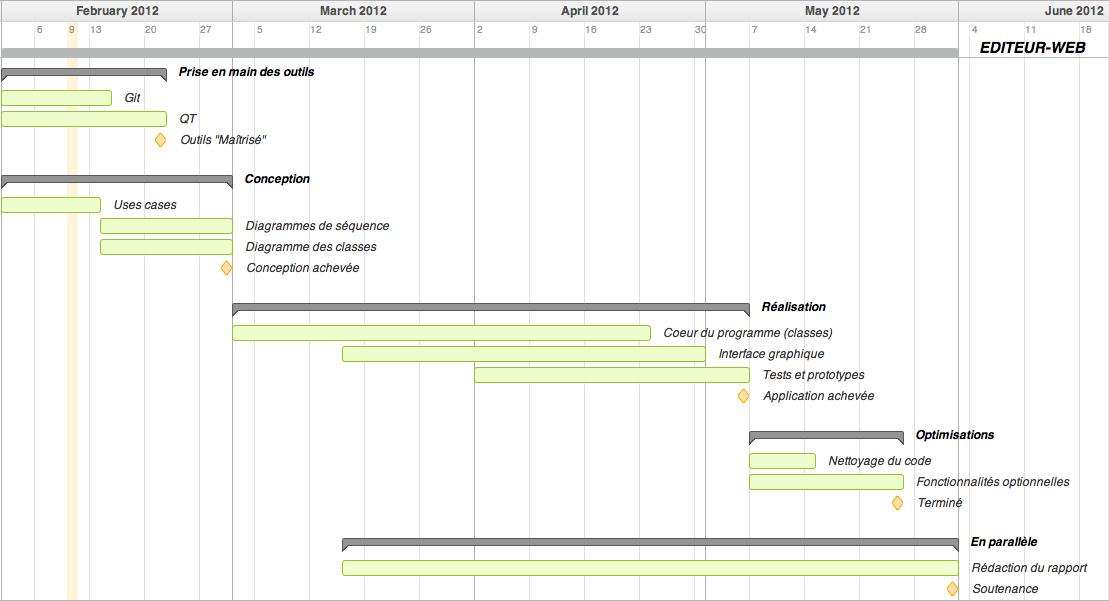
\includegraphics[width=17cm]{images/DiagrammeGantt.png}
						\caption{Diagramme de Gantt}
					\end{center}
				\end{figure}~\\
			\end{section}
		\end{chapter}
	\end{part}
%%%%%%%%%%%%%%%%%%%%%%%%%%%%%%%%%%%%%%%%
%%%%%%%%%%%%%%%%%%%%%%%%%%%%%%%%%%%%%%%%
	\begin{part}{Conception}
		\begin{chapter}{Décomposition en sous systèmes}
			Le programme se découpe grossièrement en trois sous-systèmes complémentaires comme sur le diagramme \ref{poulpe}.
			\begin{figure}[h]
				\begin{center}
					\includegraphics[width=17cm]{images/DecompositionSousSystemes.jpg}
					\caption{Décomposition en sous systèmes}
					\label{poulpe}
				\end{center}
			\end{figure}~\\
			Le système de gestion des fichiers est un système très important de l'application et c'est pourquoi il est requis
			par le système de gestion des projets.\\
			Le système de gestion du code est vue comme une extension aux fichiers. En effet, il serait possible d'éditer un
			site web sans gérer la coloration, l'indentation et toutes les fonctionnalités qui rendent un éditeur de code si agréable à utiliser.
			
			\begin{section}{Gestion des projets}
				Le sous-système de gestion des projets est un élément important de l'application, en ce sens qu'il permet à l'utilisateur
				de bien s'organiser de manière simple et efficace.\\
				À la manière de beaucoup de logiciels connus, il sera nécessaire à l'utilisateur de sélectionner un Espace de Travail,
				regroupant un ensemble de projets. Cette petite obligation n'est que très peu contraignante et favorise l'organisation, 
				sans pour autant l'imposer réellement à l'utilisateur puisque l'emplacement de cet espace de travail est donné par l'utilisateur.\\
				Un projet est concrètement représenté par un dossier sur la machine de l'utilisateur. Partant de cette idée, notre système
				de gestion de projet sera implémenté en utilisant les normes et références communément admises en termes de création,
				modification et destruction de dossiers.\\~\\
				Comme exposé ci-dessous, l'utilisateur doit pouvoir effectuer les actions classiques relatives à un projet, à savoir création, 
				modification, suppression, ouverture et fermeture, mais il peut également, comme stipulé dans le cahier des charges, 
				créer un nouveau projet basé sur un squelette de site pré-existant.\\
				Ce dernier cas de figure, non obligatoire, permet à un utilisateur d'avoir un aperçu de ce que peut être un projet de 
				site internet en développement sous notre application.\\
				L'unique caractéristique d'un projet est que l'on pourra trouver à la racine un fichier spécial résumant les paramètres utilisateur,
				les caractéristiques du projet, et autres informations diverses.\\
				Relativement à un projet, l'application fournit les fonctionnalités décrites dans le diagramme \ref{marchandise}
				\begin{figure}[ht]
					\begin{center}
						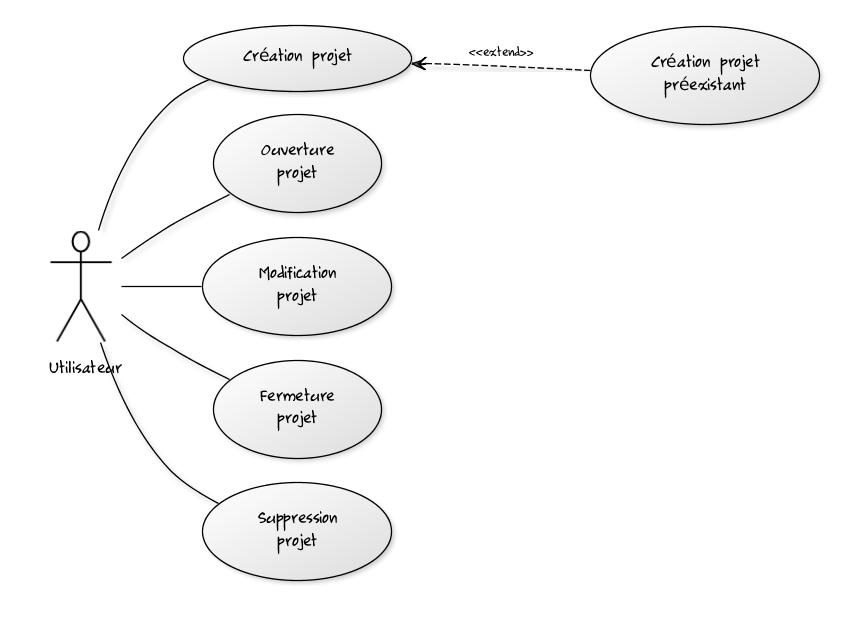
\includegraphics[width=13cm]{images/gestionProjets.jpg}
						\caption{Sous système de gestion des projets}
						\label{marchandise}
					\end{center}
				\end{figure}~\\
				À noter que cette méthode d'utilisation de l'application nous a principalement été inspirée
				par des logiciels que nous utilisons tous en cours et chez nous, comme Eclipse par exemple.\\
				À ces actions d'ordre "général" s'ajoutent quelques actions propres à la modélisation physique des projets dans notre application,
				qui sont exposées dans le diagramme \ref{ucgp}
				\begin{figure}[h]
					\begin{center}
						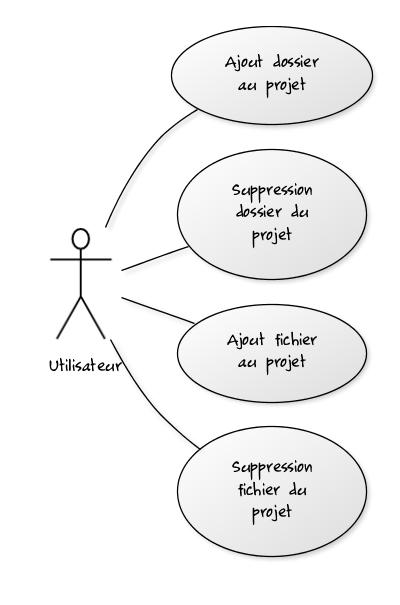
\includegraphics[height=7cm]{images/modificationProjet.jpg}
						\caption{Use-Case modification de projets}
						\label{ucgp}
					\end{center}
				\end{figure}~\\

				Ainsi comme exposé dans ce diagramme, l'utilisateur pourra créer autant de fichiers et de dossiers qu'il le souhaite dans 
				sont projet, lui permettant ainsi de pouvoir organiser son travail comme il le souhaite, plutôt que devoir se plier à un 
				mode d'organisation imposé par l'application.\\
				Toutefois, ces actions d'apparences basiques sont signes d'un travail important à venir puisqu'elles constituent des libertés
				supplémentaires	accordées à l'utilisateur.\\
			\end{section}
			\newpage
			\begin{section}{Gestion des fichiers}
			
				Le sous-système de gestion des fichiers constitue également une partie importante et consistante de notre projet, il fait
				d'ailleurs parti d'un des trois axes principaux que nous avons défini afin de pouvoir diviser notre groupe de 8 personnes en sous
				groupes à effectifs réduits.\\
				Comme pour les projets, l'application doit permettre d'effectuer des actions basiques en terme de manipulation de fichiers :
				création, ouverture, etc...\\
				L'application jouera cependant un rôle particulier au niveau de l'édition d'un fichier, puisque c'est à ce niveau qu'interviendront
				les moyens de coloration, d'indentation et d'auto-complétion du code, représenté par l'action de "gestion du code" dans le 
				diagramme \ref{ssgf} \\
				\begin{figure}[ht]
					\begin{center}
						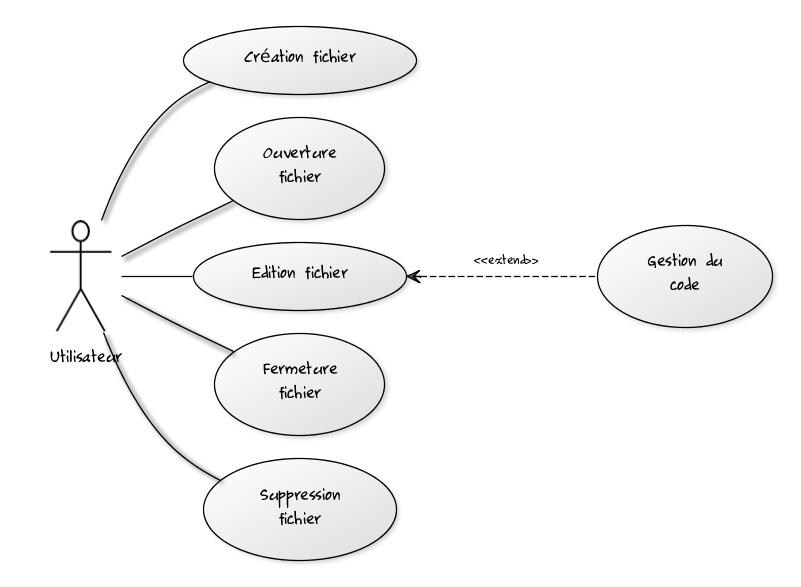
\includegraphics[width=13cm]{images/gestionFichiers.jpg}
						\caption{Sous système de gestion des fichiers}
						\label{ssgf}
					\end{center}
				\end{figure}~\\
			\end{section}

			\begin{section}{Gestion du code}
				Derrière ce nom quelque peu singulier se cache un concept fort simple, la gestion du code consiste à indenter, colorer,
				visualiser et sublimer le code source présent dans un fichier. Le diagramme \ref{saphir} parle de lui même.
				\begin{figure}[ht]
					\begin{center}
						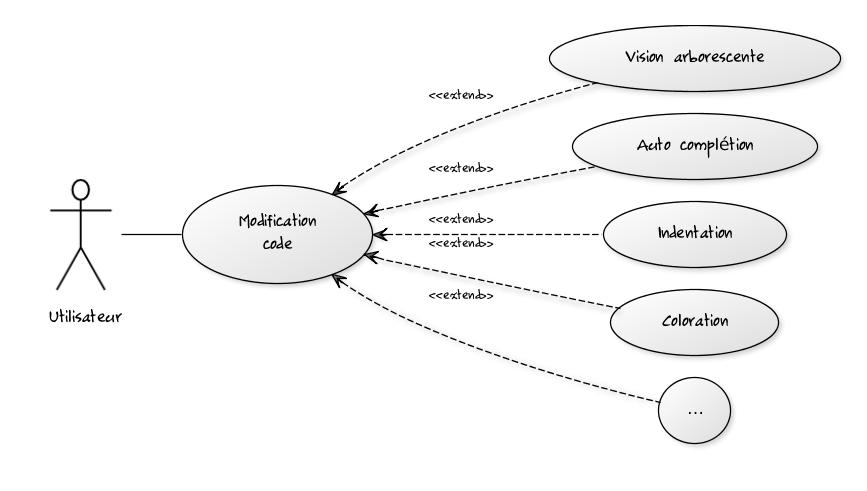
\includegraphics[width=13cm]{images/gestionCode.jpg}
						\caption{Sous système de gestion du code}
						\label{saphir}
					\end{center}
				\end{figure}~\\
			\end{section}
		\end{chapter}
		\begin{chapter}{Diagrammes des classes}
			\begin{section}{Coloration}
				La conception de la partie « coloration syntaxique » de notre application a requis l'introduction de plusieurs classes différentes.
				Premièrement des classes dites de données, suffixées du mot anglais \emph{data}, qui contiennent les différents mots clés relatifs
				à chaque langage sous forme d'\glspl{expression régulière}.\\
				Dans le diagramme \ref{blouson}, nous donnons en exemple une seule classe \emph{HtmlData}, car les autres sont similaires,
				aux particularités du langage près.
				\begin{figure}[ht]
					\begin{center}
						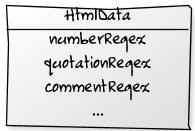
\includegraphics[width=3cm]{images/classesColorationData.jpg}
						\caption{Classe de données pour le langage Html}
						\label{blouson}
					\end{center}
				\end{figure}~\\
				De la même manière, on trouve les classes \emph{CssData, PhpData et JavaScriptData}.\\


				Une autre part de la coloration est l'utilisation concrète des classes décrites précédemment. Sur le diagramme \ref{bicyclette} sont
				représentées toutes les classes qui permettent la coloration à l'écran. Elles héritent d'une superclasse
				\emph{Highlighter} qui factorise la méthode \emph{highlightBlock()}, celle-ci, comme son nom l'indique, colore le texte bloc
				par bloc en fonction des règles données dans les classes \emph{Data}.
				\begin{figure}[ht]
					\begin{center}
						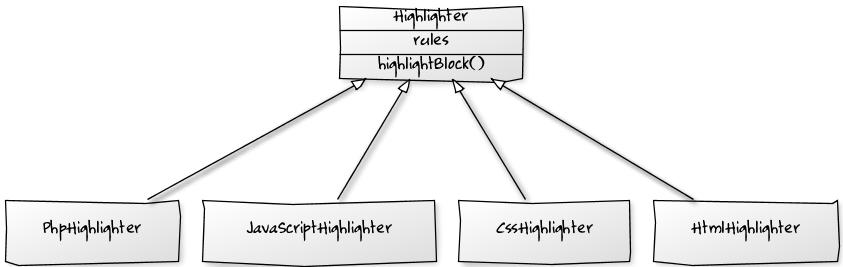
\includegraphics[width=14cm]{images/classesColoration.jpg}
						\caption{Classes de coloration}
						\label{bicyclette}
					\end{center}
				\end{figure}~\\
			\end{section}
			\begin{section}
			\end{section}
		\end{chapter}
		\begin{chapter}{Premiers pas vers la programmation}
			\begin{section}{Partage du travail et homogénéisation}
				Quelques mots sur le partage du boulot, comme on a fait, comment c'est difficile de diviser, qu'est-ce que ça apporte, blablabla
				On ajoute quelques phrases pour dire qu'on a du se mettre d'accord pour des conventions de nommage (minuscule en début de variable
				et fonctions, majuscules pour classes, etc...), pour le fait qu'on code en anglais, etc etc
				Il faut aussi faire croire que c'est à ce moment là qu'on a choisi comment documenter notre code, meme si c'est pas vrai.
			\end
			\begin{section}{Organisation du code : Le modèle MVC}
				Avant de réellement commencer la programmation, il nous a fallu parler de la façon dont nous allions organiser notre code.
				Plutôt que d'opter pour une organisation basique se contentant de dossiers "Classes", "Packages", etc... Nous avons choisi de 
				nous tourner vers une organisation dite "Modèle-Vue-Controleur", actuellement très utilisée en programmation.
			\end{section}
		\end{chapter}
	\end{part}
%%%%%%%%%%%%%%%%%%%%%%%%%%%%%%%%%%%%%%%%
%%%%%%%%%%%%%%%%%%%%%%%%%%%%%%%%%%%%%%%%
	\begin{part}{L'oeuvre}
		\begin{chapter}{Travail de groupe}
			Là on parle des réunions, pourquoi pas mettre un extrait de journal.
		\end{chapter}
		\begin{chapter}{Implémentation}
			\begin{section}{Noyau}
			\end{section}
			\begin{section}{Interface}
			\end{section}
			Ici on aborde les problèmes de la documentation, de nouvelles bibliothèques, de mettre en place nos algorithmes ``en vrai'', ... 
		\end{chapter}
		\begin{chapter}{Résultat}
			On va essayer de caser des trucs ici.
		\end{chapter}
		\begin{chapter}{Discussion}
			Critique (positive) du résultat, le cahier des charges est-il respecté ? améliorations possibles, erreurs qu'on à pu faire.
		\end{chapter}
	\end{part}
%%%%%%%%%%%%%%%%%%%%%%%%%%%%%%%%%%%%%%%%
%%%%%%%%%%%%%%%%%%%%%%%%%%%%%%%%%%%%%%%%
	\begin{chapter}*{Conclusion}
		Oué on s'est bien marré et tout et tout.lol!!!!
	\end{chapter}
%%%%%%%%%%%%%%%%%%%%%%%%%%%%%%%%%%%%%%%%
%%%%%%%%%%%%%%%%%%%%%%%%%%%%%%%%%%%%%%%%
	%% Glossaire
	\renewcommand\glossaryname{Glossaire}
	\renewcommand{\glsnamefont}[1]{\makefirstuc{#1}} % Majuscules.
	\printglossaries
%%%%%%%%%%%%%%%%%%%%%%%%%%%%%%%%%%%%%%%%
%%%%%%%%%%%%%%%%%%%%%%%%%%%%%%%%%%%%%%%%
	%% Sitographie
	\renewcommand\bibname{Sitographie}%% Changement du titre de bibliographie en sitographie.
	\begin{thebibliography}{2}
		\label{sitographie}
		\bibitem{Wikipedia}
		Wikipédia: www.wikipedia.org \\
		L'encyclopédie en ligne de laquelle j'ai tiré certaines définitions présentes dans le glossaire.
		~\\
		\bibitem{yUML}
		yUML: www.yuml.me \\
		Ce site permet de générer à la volée des diagrammes \gls{UML}, extrêmement utile lorsqu'il s'agit de travail de groupe.
		~\\
		\bibitem{Micromobs}
		Micromobs: www.micromobs.com \\
		Le site de discussion de groupe au principe intéressant: il vaut mieux une interface dédiée aux discussions plutôt
		qu'une boîte e-mail encombrée et mal organisée.
		~\\
		\bibitem{TeamGantt}
		TeamGantt: www.teamgantt.com \\
		Création en ligne de diagrammes de Gantt beaux et lisibles.
		~\\
		\bibitem{Facebook}
		Facebook: www.facebook.com \\
		Le réseau social que l'on ne présente plus, il nous a permis d'échanger des messages moins techniques que sur Micromobs
		et de nous organiser grâce à différents évènements.
	\end{thebibliography}
\end{document}
